
\documentclass[a4paper]{article}
\usepackage[utf8]{inputenc}

\usepackage[english,german]{babel} 
\usepackage[utf8]{inputenc}

\usepackage{alltt}
\usepackage{amsmath}
\usepackage{amssymb}
\usepackage{amsthm}
\usepackage{color}
\usepackage{enumitem}
\usepackage{epsfig}
\usepackage{fancyhdr}
\usepackage{float}
\usepackage{framed}
\usepackage{graphicx} 
\usepackage{graphics}
\usepackage{hyperref}
\usepackage{listings}
\usepackage{multirow}
\usepackage{tabularx}
\usepackage{textcomp}
\usepackage{tikz}
\usepackage{url}
\usepackage{vmargin}
\usepackage{xspace}
\usepackage{comment}
\usetikzlibrary{calc,trees,positioning,arrows,chains,shapes.geometric,%
    decorations.pathreplacing,decorations.pathmorphing,shapes,%
    matrix,shapes.symbols,topaths,matrix}
\newcommand{\question}[2][0]{\section{{#2} \hfill ({#1} P.)}}
\setpapersize{A4}
\setmargins{2.5cm}{2.0cm}% % linker & oberer Rand
         {16cm}{22cm}%   % Textbreite und -hoehe
           {48pt}{36pt}%   % Kopfzeilenhoehe und -abstand
           {0pt}{30pt}%    % \footheight (egal) und Fusszeilenabstand

\frenchspacing
\pagestyle{fancy}
\sloppy

\newcommand{\hide}[1]{}

\markright{Kopfzeile}


\tikzset{
>=stealth',
  punktchain/.style={
    rectangle,
    rounded corners,
    % fill=black!10,
    draw=black, very thick,
    text width=10em,
    minimum height=3em,
    text centered,
    on chain},
  line/.style={draw, thick, <-},
  element/.style={
    tape,
    top color=white,
    bottom color=blue!50!black!60!,
    minimum width=8em,
    draw=blue!40!black!90, very thick,
    text width=10em,
    minimum height=3.5em,
    text centered,
    on chain},
  every join/.style={->, thick,shorten >=1pt},
  decoration={brace},
  tuborg/.style={decorate},
  tubnode/.style={midway, right=2pt},
}


\setlength{\parindent}{0pt}
\setlength{\parskip}{5pt}
\fboxsep1.5mm


\lstdefinestyle{mystyle}{
    backgroundcolor=\color{white},   
    commentstyle=\color{codegray},
    keywordstyle=\bf \ttfamily \color{codepurple},
    numberstyle=\tiny\color{codegray},
    stringstyle=\color{codegreen},
    basicstyle=\footnotesize,
    breakatwhitespace=false,         
    breaklines=true,                 
    captionpos=b,                    
    keepspaces=true,                 
    numbers=left,                    
    numbersep=5pt,                  
    showspaces=false,                
    showstringspaces=false,
    showtabs=false,                  
    tabsize=8,
    keepspaces,
    extendedchars=true, 
      upquote=true,
    columns=fixed,
    showstringspaces=false,
    extendedchars=true,
    breaklines=true,
    frame=single,
    showspaces=false,
    showstringspaces=false,
    rulecolor=\color{white},
}

\lstdefinelanguage{sql}[]{}{
        %tag=[s]<>,      % =*: also apply styles within tag, =**: cumulate styles
        morekeywords={sql, VIEW, AS, FROM, SELECT, WHERE, FUNCTION, BOOLEAN, RETURNS, DETERMINISTIC, RETURN, REFERENCES, WITH, SEQUENCE, TRUNCATE, START, CREATE, AS, LANGUAGE, FUNCTION, CURSOR, PREPARE, OPEN, USING, CLOSE, DECLARE, END, BEGIN, EXEC, SQL, CONNECT TO, DISCONNECT, COMMIT, LOOP, IF, THEN, ELSE, WHILE, BREAK, EXIT, INSERT, INTO, VALUES, UPDATE, SET, TABLE, PRIMARY, KEY, AND, UNION, ALL, JOIN, ON, GROUP, BY, MATERIALIZED, INT, DATE, COUNT, ORDER, OVER, PARTITION, ASC, DESC, VARCHAR, NOT, NULL, PRIMARY, KEY, DECIMAL, SUM, AVG, ROWS, BETWEEN, PRECEDING, CURRENT, ROW, INSTEAD, TRIGGER, OF, FOR, EACH, EXECUTE, PROCEDURE, DISTINCT, HAVING, LIMIT},
morestring=[s]{'}{'},
morecomment=[l]{--}
        %sensitive=false
}

\lstset{style=mystyle,numbers=none,basicstyle=\ttfamily,upquote=true}

 
\definecolor{codegreen}{rgb}{0,0.6,0}
\definecolor{codegray}{rgb}{0.5,0.5,0.5}
\definecolor{codepurple}{rgb}{0.38,0,0.72}
\definecolor{backcolour}{rgb}{0.95,0.95,0.92}
\definecolor{backcolourSingleCode}{rgb}{0.95,0.95,0.92}

\newcommand{\subtitle}{\textbf{Exercise 9}}
\newcommand{\outdate}{08.01.2024}
\newcommand{\duedate}{15.01.2024 12:00 MEZ}
\newcommand{\video}{049}

\begin{document}

\lhead{\begin{tabular}{l}
{\bf Database Systems WS 2023/24}\\
{\bf \subtitle: Distributed \outdate, Due \duedate}\\
{Submitted by }
\end{tabular}
}
\rhead{}

\question[1]{Skyline Queries}

Given the TPC-H\footnote{\url{http://dbis.informatik.uni-kl.de/files/teaching/ws1819/dbs/protected/tpch.dmp.gz}} table \textbf{''part''}.

We want to compute the skyline over the following four dimensions:
\begin{itemize}
\item \emph{p\_size:} larger is better,
\item \emph{p\_retailprice:} less is better,
\item \emph{p\_container:} Use the function \texttt{getContainerSize} from below: less is better.
\item \emph{p\_brand:} Cannot be compared.
\end{itemize}

In OLAT you will find a file \texttt{skylineFunc.sql}, which implements the \texttt{getContainerSize} function.
You can either copy the create-statement from the file and execute it in your DBMS or you can directly execute the file with the following command (you may have to change the database name to the one you used to create it).
\begin{verbatim}
psql -d tpch -f skylineFunc.sql
\end{verbatim} 

\begin{enumerate}
\item Create a SQL query to calculate the number of elements in the skyline defined above (without using the \verb+SKYLINE+-operator).
Submit the query and the result.\\\\
{\bf Solution:}\\
\begin{lstlisting}[language=sql]
SELECT COUNT(*) 
FROM part p
WHERE NOT EXISTS(
SELECT *
FROM part p1
WHERE p1.p_size >= p.p_size
AND p1.p_retailprice <= p.p_retailprice
AND getContainerSize(p1.p_container) <= getContainerSize(p.p_container)
AND p1.p_brand = p.p_brand
AND (p1.p_size > p.p_size OR p1.p_retailprice < p.p_retailprice OR getContainerSize(p1.p_container) < getContainerSize(p.p_container)))
\end{lstlisting}

The output of the query is 250.


\item Write the same query using the \verb+SKYLINE+-operator. (You do not have to install the plugin and execute the query.)\\\\
{\bf Solution:}\\
\begin{lstlisting}[language=sql]
SELECT COUNT(*) 
FROM part p
SKYLINE OF p.p_size MAX, p.p_retailprice MIN, 
  getContainerSize(p.p_container) MIN, p.p_brand DIFF;
\end{lstlisting}

\end{enumerate}

\question[1]{Skyline NN}

Implement the nearest neighbor (NN) method to compute skylines in a language of your choice. A basic Java template is available in OLAT.
This template provides a (fake) R-Tree implementation which can be used to query for the nearest neighbor of a point, all points within a rectangle, and the nearest neighbor within a rectangle.
If you are using another language, you are allowed to also implement a fake R-Tree with the methods described above (or use a real implementation without a included skyline function).

The program should output the calculated skyline (the template already takes care of this).

Submit your code and the output for the following points (If you use the template, the points are already included):

$$(10,20),(12,10),(8,11),(16,19),(6,4),(5,6),(14,12),(2,5),(3,10),(13,19),(17,5),(9,3),(20,8),(8,10)$$
\\\\
{\bf Solution:}\\
\begin{figure}[H]
  \centering
  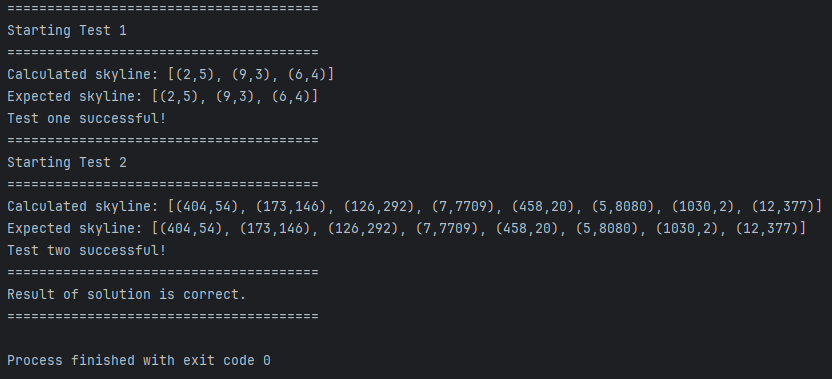
\includegraphics[scale = 0.6]{SkylineOutput.png}
\end{figure}

\newpage

\question[1]{Transactions}

\begin{enumerate}
	\item A database has the consistency condition $0\leq A\leq B$. Describe, for the following transactions, if the condition is fulfilled. Explain your answer.

    \begin{enumerate}

    \item[$T_1: $] \quad {\tt B:= 2*A; A:= 2*B;}
    \item[$T_2: $] \quad {\tt B:= A+1; A:= B+1;}
    \item[$T_3: $] \quad {\tt A:= A+2*B; B:= 2*A+B;}
    \end{enumerate}

\item For each of the previous transactions, provide the input, read, and write operations. Assume immediate write-back of the changed values. Describe the effect of these operations on the main memory and the hard disk. The initial values are $A=5$ and $B=10$.

\item Given two transactions $T_1$ and $T_2$ and the following situation (' marks changed entries):

 \begin{center}

    \begin{tikzpicture}

      \draw (0,0) -- (6,0) -- (6,5.5) -- (0,5.5) -- (0,0);
      \draw (0,1) -- (6,1); \draw (0,2.5) -- (6,2.5); \draw (0,3.5) -- (6,3.5); \draw (0,4.5) -- (6,4.5);
      \draw (2,0) -- (2,1); \draw (4,0) -- (4,1);
      \draw (2,2.5) -- (2,5.5); \draw (4,2.5) -- (4,5.5);
      \node at (3,2) {\dots};

      \node at (10,2.5) [cylinder, shape border rotate=90, draw,minimum height=5cm,minimum width=4cm] {};

      \node at (3,6) {DBMS Buffer, e.g., Main Memory};
      \node at (10,6) {External Memory, e.g., Hard Disk};
      \draw[->] (8,4) -- (6.1,4) node[midway, above] {\footnotesize Insertion};
      \draw[->] (6.1,2) -- (8,2) node[midway, below] {\footnotesize Removal};

      \node at (2.5, 4) {$A^\prime$};
      \node at (3.5, 4) {$D^\prime$};
      \node at (1, 3) {$C^\prime$};
      \node at (3, 0.5) {$B$};

      \draw (9,3.5) -- (11,3.5) -- (11,4.5) -- (9,4.5) -- (9,3.5);
      \node at (8.5,4.5) {$P_A$};
      \node at (9.5,4) {$A^\prime$};
      \node at (10.5,4) {$D$};

      \draw (8.5,2.2) -- (10.5,2.2) -- (10.5,3.2) -- (8.5,3.2) -- (8.5,2.2);
      \node at (8.25,3.2) {$P_C$};
      \node at (9.5,2.7) {$C^\prime$};

      \draw (9.7,0.5) -- (11.7,0.5) -- (11.7,1.5) -- (9.7,1.5) -- (9.7,0.5);
      \node at (9.4,1.4) {$P_B$};
      \node at (10.5,1) {$B$};
    \end{tikzpicture}
  \end{center}
  \vspace{-0.15cm}

The following table describes the operations of $T_1$ and $T_2$ at different times. \\[0mm]

\vspace{-0.15cm}

\begin{center}
\begin{tabular}{r|rr} 
\multicolumn{1}{r}{Time} & \multicolumn{1}{c}{$T_1$} & \multicolumn{1}{c}{$T_2$} \\ \hline
\multicolumn{3}{c}{} \\
\ 0 & READ(A,a)  & READ(C,c) \\
10  & a:=a+10    & c:=c*2 \\
20  &            & READ(B,b) \\
30  & WRITE(A,a) &  \\
40  & READ(D,d)  & b:=b+c/4 \\
50  & d:=17*d+42 &  \\
60  & OUTPUT(A)  & WRITE(C,c) \\
70  & WRITE(D,d) & OUTPUT(C) \\
80  & OUTPUT(D)  & WRITE(B,b) \\
90  & COMMIT     & \\
100  &            & COMMIT \\
\end{tabular} \\[10mm]
\end{center}

Discuss if the illustration matches the entries of the table. Does it only represent the table at a specific time (if yes, when and why) or does it not represent it at all?

If the system crashes during the execution, what would have to be done to guarantee ACID?
Which parts of ACID are affected?
How does the situation change at timestamp 101?

\end{enumerate}

\newpage
\question[1]{Recovery}

In a DBMS three transactions $T_1,T_2$, and $T_3$ are executed concurrently. The data accessed performed by the transactions are stored in the log (Table~\ref{tab:log}).

\begin{enumerate}
  \item The system crashes after step $19$. None of the changes were written to the database, but the log is complete. Using this log, perform the three stages of recovery and explain what happens. 
  Explain your steps in-detail.

  \item Is the log changed after completing the recovery process? If yes, explain what changed.

\end{enumerate}

\begin{center}
  \begin{table}[h]
  \begin{tabular}{|l|l|l|l|l|}
  \hline      & $T_1$     & $T_2$   & $T_3$   & Log  \\ 
  \hline      &           &         &         & [LSN, TA,   PageID, Redo,     Undo,       PrevLSN]\\ 
  1. & $BOT $ & $ $ & $ $ & $[\#01, T_1, -, BOT, -, 0] $ \\ 
2. & $r(B,B_1) $ & $ $ & $ $ & $ $ \\ 
3. & $B_1 = B_1 * 8 $ & $ $ & $ $ & $ $ \\ 
4. & $ $ & $BOT $ & $ $ & $[\#02, T_2, -, BOT, -, 0] $ \\ 
5. & $w(B,B_1) $ & $ $ & $ $ & $[\#03, T_1, P_B, B = B * 8, B = B / 8, \#01] $ \\ 
6. & $ $ & $r(A,A_1) $ & $ $ & $ $ \\ 
7. & $ $ & $ $ & $BOT $ & $[\#04, T_3, -, BOT, -, 0] $ \\ 
8. & $ $ & $A_1 = A_1 + 9 $ & $ $ & $ $ \\ 
9. & $ $ & $w(A,A_1) $ & $ $ & $[\#05, T_2, P_A, A = A + 9, A = A - 9, \#02] $ \\ 
10. & $abort $ & $ $ & $ $ & $[\#06, T_1, -, abort, -, \#03] $ \\ 
11. & $ $ & $r(C,C_1) $ & $ $ & $ $ \\ 
12. & $ $ & $ $ & $r(A,A_2) $ & $ $ \\ 
13. & $ $ & $ $ & $A_2 = A_2 + 3 $ & $ $ \\ 
14. & $ $ & $C_1 = C_1 / 1 $ & $ $ & $ $ \\ 
15. & $ $ & $w(C,C_1) $ & $ $ & $[\#07, T_2, P_C, C = C / 1, C = C * 1, \#05] $ \\ 
16. & $ $ & $commit $ & $ $ & $[\#08, T_2, -, commit, -, \#07] $ \\ 
17. & $ $ & $ $ & $w(A,A_2) $ & $[\#09, T_3, P_A, A = A + 3, A = A - 3, \#04] $ \\ 
18. & $ $ & $ $ & $r(B,B_2) $ & $ $ \\ 
19. & $ $ & $ $ & $B_2 = B_2 / 6 $ & $ $ \\ 
\hline      &       &       &     &\textbf{Crash} \\  
  \hline 
  \end{tabular}
  \caption{Log}
  \label{tab:log}
  \end{table}
  \end{center}

\end{document}
